\documentclass{beamer}
\usepackage[utf8]{inputenc}
\usetheme{Madrid}
\usecolortheme{default}
\usepackage{amsmath,amssymb,amsfonts,amsthm}
\usepackage{txfonts}
\usepackage{tkz-euclide}
\usepackage{listings}
\usepackage{adjustbox}
\usepackage{array}
\usepackage{tabularx}
\usepackage{gvv}
\usepackage{lmodern}
\usepackage{circuitikz}
\usepackage{tikz}
\usepackage{graphicx}
\setbeamertemplate{page number in head/foot}[totalframenumber]
\usepackage{tcolorbox}
\tcbuselibrary{minted,breakable,xparse,skins}
\definecolor{bg}{gray}{0.95}
\DeclareTCBListing{mintedbox}{O{}m!O{}}{%
  breakable=true,
  listing engine=minted,
  listing only,
  minted language=#2,
  minted style=default,
  minted options={%
    linenos,
    gobble=0,
    breaklines=true,
    breakafter=,,
    fontsize=\small,
    numbersep=8pt,
    #1},
  boxsep=0pt,
  left skip=0pt,
  right skip=0pt,
  left=25pt,
  right=0pt,
  top=3pt,
  bottom=3pt,
  arc=5pt,
  leftrule=0pt,
  rightrule=0pt,
  bottomrule=2pt,
  toprule=2pt,
  colback=bg,
  colframe=orange!70,
  enhanced,
  overlay={%
    \begin{tcbclipinterior}
    \fill[orange!20!white] (frame.south west) rectangle ([xshift=20pt]frame.north west);
    \end{tcbclipinterior}},
  #3,
}
\lstset{
    language=C,
    basicstyle=\ttfamily\small,
    keywordstyle=\color{blue},
    stringstyle=\color{orange},
    commentstyle=\color{green!60!black},
    numbers=left,
    numberstyle=\tiny\color{gray},
    breaklines=true,
    showstringspaces=false,
}
\begin{document}

\title 
{9.2.27}
\date{september 2025}


\author 
{Namaswi-EE25BTECH11060}
\frame{\titlepage}
\begin{frame}{Question}
Find the Area enclosed by the parabola $4y=3x^2$ and the Line 2y=3x+12
\end{frame}
 \begin{frame}{Solution}
     Given Line 
\begin{align}
2y=3x+12\\
\vec{x}=\vec{h}+k\vec{m} ; k \in \mathbb{R}\\
\vec{h} = \begin{pmatrix} 0 \\ 6 \end{pmatrix}\\ \quad 
\vec{m} = \begin{pmatrix} 2 \\ 3 \end{pmatrix}
\end{align}
 \end{frame}
 \begin{frame}{Solution}
     Given curve
\begin{align}
    4y=3 x^2\\
    \vec{x}^\top \vec{V} \vec{x} + 2\vec{u}^\top \vec{x} + f = 0\\
    \vec{V} = \begin{pmatrix} 3 & 0 \\ 0 & 0 \end{pmatrix}\\ \quad
\vec{u} = \begin{pmatrix} 0 \\ -2 \end{pmatrix} \\ \quad
f = 0
\end{align}
 \end{frame}
 \begin{frame}{Solution}
     Points of Intersection\\
\begin{align}
    \kappa_i = \frac{1}{\vec{m}^\top \vec{V} \vec{m}} 
\left( -\vec{m}^\top (\vec{V}\vec{h} + \vec{u}) 
\pm \sqrt{ \left[ \vec{m}^\top (\vec{V}\vec{h} + \vec{u}) \right]^2 
- g(\vec{h}) \cdot (\vec{m}^\top \vec{V} \vec{m}) } \right)
\end{align}
where
\begin{align}
    g(\vec{h}) = \vec{h}^\top \vec{V} \vec{h} 
+ 2\vec{u}^\top \vec{h} + f\\
\end{align}
 \end{frame}
 \begin{frame}{Solution}
     \begin{align}
         \vec{V}\vec{h} &= \begin{pmatrix} 3 & 0 \\ 0 & 0 \end{pmatrix}
\begin{pmatrix} 0 \\ 6 \end{pmatrix} = \begin{pmatrix} 0 \\ 0 \end{pmatrix} \\
\vec{V}\vec{h} + \vec{u} &= \begin{pmatrix} 0 \\ -2 \end{pmatrix} \\
\vec{m}^\top (\vec{V}\vec{h} + \vec{u}) &= 
\begin{pmatrix} 2 & 3 \end{pmatrix} \begin{pmatrix} 0 \\ -2 \end{pmatrix} 
= -6 \\
\vec{m}^\top \vec{V} \vec{m} &= 
\begin{pmatrix} 2 & 3 \end{pmatrix} 
\begin{pmatrix} 3 & 0 \\ 0 & 0 \end{pmatrix} 
\begin{pmatrix} 2 \\ 3 \end{pmatrix} = 
\begin{pmatrix} 2 & 3 \end{pmatrix} \begin{pmatrix} 6 \\ 0 \end{pmatrix} = 12 \\
\vec{u}^\top \vec{h} &= 
\begin{pmatrix} 0 & -2 \end{pmatrix} \begin{pmatrix} 0 \\ 6 \end{pmatrix} = -12 \\
g(\vec{h}) &= 0 + 2(-12) + 0 = -24
     \end{align}
 \end{frame}
 \begin{frame}{Solution}
     \begin{align}
         \kappa_i &= \frac{1}{12} \left(6 \pm \sqrt{(-6)^2 - (-24)(12)}\right) \\
&= \frac{1}{12} \left(6 \pm \sqrt{36 + 288}\right) \\
&= \frac{1}{12} \left(6 \pm \sqrt{324}\right)\\ 
=\frac{1}{12} (6 \pm 18)\\
= \kappa_1 = \frac{24}{12} = 2, \quad 
\kappa_2 = \frac{-12}{12} = -1
\end{align}
The point of intersection are :
\begin{align}
    (4, 12) \quad \text{and} \quad (-2, 3)
\end{align}
 \end{frame}
 \begin{frame}{Solution}
     Area Bounded by curves is given by \\
\begin{align}
   \left | \int_{-2}^{4} \frac{3x^2}{4}-\frac{3x+12}{2} \right |\\
   = \left |\frac{1}{4}\int_{-2}^{4} 3 x^2 -6x -24  \right |\\
   = \left |\frac{1}{4}\brak{ x^3 -3 x^2 -24 x }_{-2}^{4} \right |\\
   =\left | \frac{1}{4}\brak{4^3 - (-2)^3 -3(4^2 - (-2)^2) -24(4-(-2)} \right |\\
           =27 
\end{align}
 \end{frame}
 \begin{frame}[fragile]
     \frametitle{C Code}
     \begin{lstlisting}
         #include <stdio.h>
#include <math.h>
double* compute_points_and_area() {
    static double results[5]; // results[0,1]=P1, [2,3]=P2, [4]=area

    double h[2] = {0, 6};
    double m[2] = {2, 3};
    double V[2][2] = {{3,0},{0,0}};
    double u[2] = {0, -2};
    double f = 0;
     \end{lstlisting}
 \end{frame}
  \begin{frame}[fragile]
     \frametitle{C Code}
     \begin{lstlisting}
         // Step 1: V*h + u
    double Vh[2];
    Vh[0] = V[0][0]*h[0] + V[0][1]*h[1];
    Vh[1] = V[1][0]*h[0] + V[1][1]*h[1];

    double Vh_plus_u[2] = {Vh[0]+u[0], Vh[1]+u[1]};

    // Step 2: m^T*(Vh+u)
    double mT_Vh_plus_u = m[0]*Vh_plus_u[0] + m[1]*Vh_plus_u[1];

     \end{lstlisting}
 \end{frame}
  \begin{frame}[fragile]
     \frametitle{C Code}
     \begin{lstlisting}
          // Step 3: m^T * V * m
    double Vm[2] = { V[0][0]*m[0] + V[0][1]*m[1], V[1][0]*m[0] + V[1][1]*m[1] };
    double mT_V_m = m[0]*Vm[0] + m[1]*Vm[1];

    // Step 4: g(h)
    double hT_V_h = h[0]*(V[0][0]*h[0]+V[0][1]*h[1]) + h[1]*(V[1][0]*h[0]+V[1][1]*h[1]);
    double uT_h = u[0]*h[0] + u[1]*h[1];
    double g_h = hT_V_h + 2*uT_h + f;
     \end{lstlisting}
 \end{frame}
  \begin{frame}[fragile]
     \frametitle{C Code}
     \begin{lstlisting}
         // Step 5: kappa values
    double sqrt_term = sqrt(mT_Vh_plus_u*mT_Vh_plus_u - g_h*mT_V_m);
    double kappa1 = (-mT_Vh_plus_u + sqrt_term)/mT_V_m;
    double kappa2 = (-mT_Vh_plus_u - sqrt_term)/mT_V_m;

    // Step 6: Intersection points
    results[0] = h[0] + kappa1*m[0]; // P1 x
    results[1] = h[1] + kappa1*m[1]; // P1 y
    results[2] = h[0] + kappa2*m[0]; // P2 x
    results[3] = h[1] + kappa2*m[1]; // P2 y
     \end{lstlisting}
 \end{frame}
  \begin{frame}[fragile]
     \frametitle{C Code}
     \begin{lstlisting}
         // Step 7: Area
    double x1 = results[2]; // -2
    double x2 = results[0]; // 4
    results[4] = fabs((1.0/4)*(pow(x2,3)-pow(x1,3)-3*(pow(x2,2)-pow(x1,2))-24*(x2-x1)));

    return results;
}
 \end{lstlisting}
 \end{frame}
 \begin{frame}[fragile]
 \frametitle{Python Code}
     \begin{lstlisting}
         import numpy as np
import matplotlib.pyplot as plt

# Define the x range
x = np.linspace(-5, 5, 500)

# Define the curves
y_curve = (3/4) * x**2      # 4y = 3x^2  => y = 3/4 x^2
y_line  = (3/2) * x + 6     # 2y = 3x+12 => y = 3/2 x + 6

     \end{lstlisting}
 \end{frame}
 \begin{frame}[fragile]
 \frametitle{Python Code}
     \begin{lstlisting}
        
# Plot the curves
plt.plot(x, y_curve, label=r'$4y=3x^2$', color='blue')
plt.plot(x, y_line, label=r'$2y=3x+12$', color='red')

# Find intersection points for shading
# Solve (3/4)x^2 = (3/2)x + 6  => 3x^2/4 - 3x/2 - 6 = 0
# Multiply by 4: 3x^2 - 6x - 24 = 0  => x^2 - 2x - 8 = 0
# Using quadratic formula: x = 1 ± 3
x1 = -2
x2 = 4
 
     \end{lstlisting}
 \end{frame}
 \begin{frame}[fragile]
 \frametitle{Python Code}
     \begin{lstlisting}
         
# Shade the area between the curves
x_fill = np.linspace(x1, x2, 500)
plt.fill_between(x_fill, (3/4)*x_fill**2, (3/2)*x_fill + 6, color='green', alpha=0.3, label='Shaded Area')

# Add labels, grid, and legend
plt.xlabel('x')
plt.ylabel('y')
plt.title('Area between $4y=3x^2$ and $2y=3x+12$')
plt.grid(True)
plt.legend()
plt.show()

     \end{lstlisting}
 \end{frame}
 \begin{frame}[fragile]
     \frametitle{C and Python Code}
     \begin{lstlisting}
         import ctypes
# Load the shared object
lib = ctypes.CDLL("./curves.so")

# Specify return type
lib.compute_points_and_area.restype = ctypes.POINTER(ctypes.c_double)

# Call the function
result_ptr = lib.compute_points_and_area()
results = [result_ptr[i] for i in range(5)]
     \end{lstlisting}
 \end{frame}
 \begin{frame}[fragile]
     \frametitle{C and Python Code}
     \begin{lstlisting}
         P1 = (results[0], results[1])
P2 = (results[2], results[3])
area = results[4]

print("Intersection points:")
print("P1:", P1)
print("P2:", P2)
print("Area bounded by curves:", area)

     \end{lstlisting}
 \end{frame}
\begin{frame}{plot}
     \centering
    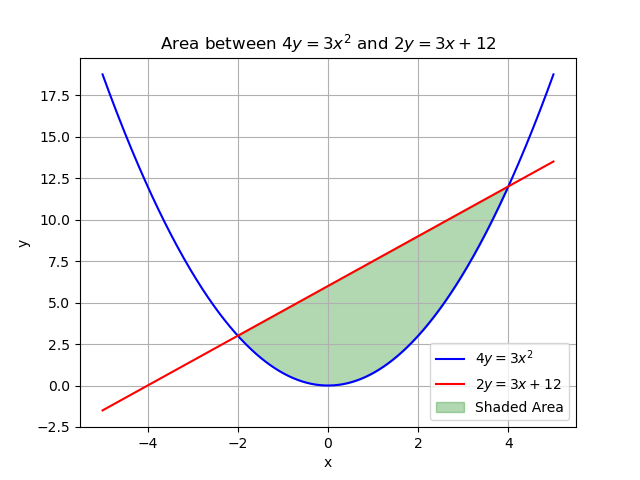
\includegraphics[width=\columnwidth, height=0.8\textheight, keepaspectratio]{Figure_15.png} 
\end{frame}
\end{document}